\chapter{Projekt rozwiązania}
\label{chap:hl-arch}

    Niniejszy rozdział przedstawia koncepcję systemu. Definiuje użytkowników oraz wymagania funkcjonalne i pozafunkcjonalne. Przedstawia budowę systemu, opisuje kolejno tworzące system komponenty sprzętowe oraz podsystemy, a także relacje, które między nimi zachodzą. Ponadto prezentuje zakładany sposób działania systemu w kilku najbardziej prawdopodobnych sytuacjach.

    \section{Idea}
        Idea systemu przedstawiona została na rysnku \ref{fig:door}.

        \begin{figure}[h!]
            \begin{center}
                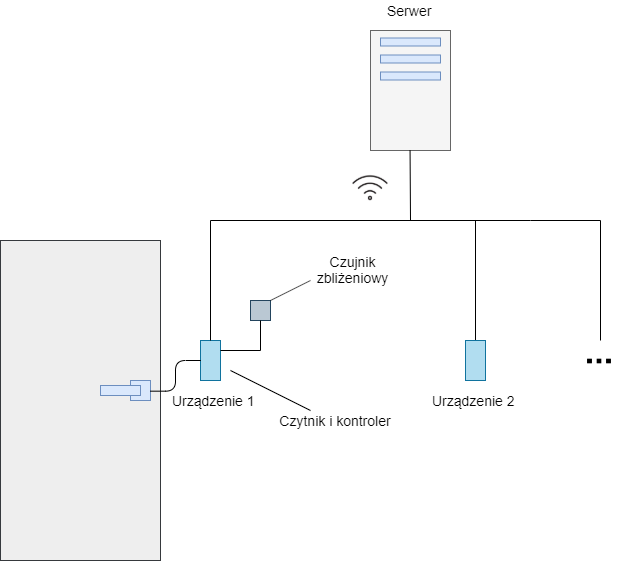
\includegraphics[width=.7\linewidth]{chapters/images/door2.png}
                \caption{Idea systemu}
                \label{fig:door}
            \end{center}
        \end{figure}

    \section{Użytkownicy}
        Na potrzeby projektu rozwiązania zidentyfikowano dwóch użytkowników. Ich specyfikacja przedstawiona została w tabeli \ref{tbl:users}.

        \begin{table}[h!]
            \caption{Użytkownicy systemu}
            \centering
            \begin{subtable}[c]{\textwidth}
                \centering
                \begin{tabular}{|p{2cm}|p{12cm}|}
                    \hline USER\_1      & \textbf{Użytkownik} \\
                    \hline \cellcolor[gray]{0.8} Opis         & Osoba posiadająca identyfikator RFID, której celem jest uzyskanie dostępu do chronionego zamkiem pomieszczenia  \\
                    \hline
                \end{tabular}
                \label{tbl:usr1}
                \vspace{10mm}           
            \end{subtable}
        \quad%
            \begin{subtable}[c]{\textwidth}
                \centering
                \begin{tabular}{|p{2cm}|p{12cm}|}
                    \hline USER\_2      & \textbf{Administrator} \\
                    \hline \cellcolor[gray]{0.8} Opis         & Osoba posiadająca uprawnienia administracyjne w systemie, mająca dostęp do oprogramowania zarządzającego systemem \\
                    \hline
                \end{tabular}
                \label{tbl:usr2}       
            \end{subtable}                
            \label{tbl:users}
        \end{table}

    \section{Wymagania}

        Wymagania funkcjonalne oraz pozafunkcjonalne systemu zostały przedstawione odpowiednio w tabeli \ref{tbl:fnrq} i \ref{tbl:xxrq}.

        \begin{table}[h!]
            \caption{Wymagania funkcjonalne}
            \centering
            \begin{subtable}[c]{\textwidth}
                \centering
                \begin{tabular}{|p{2cm}|p{12cm}|}
                    \hline FNRQ\_1      & \textbf{Kontrola dostępu do pomieszczeń}  \\
                    \hline \cellcolor[gray]{0.8} Opis         & Dopuszczanie do pomieszczeń użytkowników posiadających odpowiedni identyfikator i niedopuszczanie użytkowników nieposiadających odpowiedniego identyfikatora  \\
                    \hline
                \end{tabular}
                \label{tbl:fnrq1}
                \vspace{10mm}           
            \end{subtable}
        \quad%  
            \begin{subtable}[c]{\textwidth}
                \centering
                 \begin{tabular}{|p{2cm}|p{12cm}|}
                    \hline FNRQ\_2      & \textbf{Przeglądanie historii prób dostępu do pomieszczeń}  \\
                    \hline \cellcolor[gray]{0.8} Opis         & Dostęp do listy dokonanych w przeszłości prób dostępu zakończonych zarówno sukcesem, jak i porażką \\
                    \hline
                \end{tabular}
                \label{tbl:fnrq2}
                \vspace{10mm}           
            \end{subtable}
            \begin{subtable}[c]{\textwidth}
                \centering
                 \begin{tabular}{|p{2cm}|p{12cm}|}
                    \hline FNRQ\_3      & \textbf{Dodawanie identyfikatorów}  \\
                    \hline \cellcolor[gray]{0.8} Opis         & Dodawanie identyfikatorów wraz z przyznaniem dostępu do wybranej grupy zamków \\
                    \hline
                \end{tabular}
                \label{tbl:fnrq3}
                \vspace{10mm}           
            \end{subtable}
        \label{tbl:fnrq}
        \end{table}
    
        \pagebreak  

        \begin{table}[h!]
            \ContinuedFloat
            \caption{Wymagania funkcjonalne, c.d.}
            \begin{subtable}[c]{\textwidth}
                \centering
                 \begin{tabular}{|p{2cm}|p{12cm}|}
                    \hline FNRQ\_4      & \textbf{Przeglądanie identyfikatorów powiązanych z danym zamkiem} \\
                    \hline \cellcolor[gray]{0.8} Opis         & Dostęp do listy powiązań między identyfikatorami a zamkami \\
                    \hline
                \end{tabular}
                \label{tbl:fnrq4}
                \vspace{10mm}           
            \end{subtable}
        \quad%
            \begin{subtable}[c]{\textwidth}
                \centering
                 \begin{tabular}{|p{2cm}|p{12cm}|}
                    \hline FNRQ\_5      & \textbf{Blokowanie dostępu do pomieszczeń dla wybranego identyfikatora}  \\
                    \hline \cellcolor[gray]{0.8} Opis         & Manualny wybór opcji czasowego usunięcia powiązania wybranego identyfikatora z wybraną grupą zamków \\
                    \hline
                \end{tabular}
                \label{tbl:fnrq5}
                \vspace{10mm}           
            \end{subtable}
        \quad%
            \begin{subtable}[c]{\textwidth}
                \centering
                 \begin{tabular}{|p{2cm}|p{12cm}|}
                    \hline FNRQ\_6      & \textbf{Dostęp do grupy pomieszczeń za pomocą jednego identyfikatora}  \\
                    \hline \cellcolor[gray]{0.8} Opis         & Ustawienie powiązań identyfikatorów i zamków w taki sposób, aby możliwy był dostęp do grupy zamków za pomocą jednego identyfikatora \\
                    \hline
                \end{tabular}
                \label{tbl:fnrq6}
                \vspace{10mm}           
            \end{subtable}
        \quad%
            \begin{subtable}[c]{\textwidth}
                \centering
                 \begin{tabular}{|p{2cm}|p{12cm}|}
                    \hline FNRQ\_7      & \textbf{Dostęp do pomieszczenia za pomocą grupy identyfikatorów}  \\
                    \hline \cellcolor[gray]{0.8} Opis         & Ustawienie powiązań identyfikatorów i zamków w taki sposób, aby możliwy był dostęp do jednego zamka za pomocą grupy identyfikatorów \\
                    \hline
                \end{tabular}
                \label{tbl:fnrq7}
                \vspace{10mm}           
            \end{subtable}
        \quad%
            \begin{subtable}[c]{\textwidth}
                \centering
                 \begin{tabular}{|p{2cm}|p{12cm}|}
                    \hline FNRQ\_8      & \textbf{Sygnalizacja przyznania lub odmowy dostępu}  \\
                    \hline \cellcolor[gray]{0.8} Opis         & Powiadamianie użytkownika o podjętej przez system decyzji \\
                    \hline
                \end{tabular}
                \label{tbl:fnrq8}
                \vspace{10mm}           
            \end{subtable}
        \quad%
            \begin{subtable}[c]{\textwidth}
                \centering
                 \begin{tabular}{|p{2cm}|p{12cm}|}
                    \hline FNRQ\_9      & \textbf{Sygnalizacja stanu naładowania baterii w układzie zamka} \\
                    \hline \cellcolor[gray]{0.8} Opis         & Okresowe powiadamianie administratora systemu o bieżącym stanie naładowania baterii \\
                    \hline
                \end{tabular}
                \label{tbl:fnrq9}         
            \end{subtable}
            \label{tbl:fnrq_2}
        \end{table}

        \begin{table}[h!]
            \caption{Wymagania pozafunkcjonalne}
            \centering
            \begin{subtable}[c]{\textwidth}
                \centering
                \begin{tabular}{|p{2cm}|p{12cm}|}
                    \hline XXRQ\_1      & \textbf{Długość czasu pracy układu zamka na baterii równa minimum 1 rok}  \\
                    \hline \cellcolor[gray]{0.8} Opis         & Długość czasu pracy układu zamka na baterii powinna wynosić minimum 1 rok \\
                    \hline
                \end{tabular}
                \label{tbl:xxrq1}
                \vspace{10mm}       
            \end{subtable}
        \quad%
            \begin{subtable}[c]{\textwidth}
                \centering
                \begin{tabular}{|p{2cm}|p{12cm}|}
                    \hline XXRQ\_2      & \textbf{Czas odpowiedzi układu zamka nie dłuższy niż 3 sekundy}  \\
                    \hline \cellcolor[gray]{0.8} Opis         & Czas odpowiedzi układu zamka od momentu przyłożenia identyfikatora do momentu wysłania sygnału otwierającego zamek przez układ sterowania zamkiem powinien być nie dłuższy niż 3 sekundy. \\
                    \hline
                \end{tabular}
                \label{tbl:xxrq2}    
            \end{subtable}

            \label{tbl:xxrq}
        \end{table}

        \section{Komponenty}

            System podzielony został na podsystemy (tabela \ref{tbl:subsystems}) realizujące określone funkcjonalności za pomocą komponentów programowych (tabela \ref{tbl:sw_comp}) i istniejące w ramach fizycznych komponentów sprzętowych (tabela \ref{tbl:hw_comp}).

                \begin{table}
                    \caption{Podsystemy}
                    \centering
                    \begin{subtable}[c]{\textwidth}
                        \centering
                        \begin{tabular}{|p{2cm}|p{12cm}|}
                            \hline SSYS\_1      & \textbf{Podsystem sterowania zamkiem} \\
                            \hline \cellcolor[gray]{0.8} Opis         & Odpowiedzialny za odczyt danych identyfikatora użytkownika oraz przekazanie ich do podsystemu autoryzacji, zarządzanie zasilaniem elementów układu zamka oraz zarządzanie samym zamkiem.  \\
                            \hline \cellcolor[gray]{0.8} Lokalizacja  & HCMP\_1 Układ zamka    \\
                            \hline \cellcolor[gray]{0.8} Komponenty   & SCMP\_1 Oprogramowanie mikrokontrolera w układzie zamka    \\
                            \hline
                        \end{tabular}
                        \label{tbl:scmp1}
                        \vspace{10mm}           
                    \end{subtable}
                \quad%
                    \begin{subtable}[c]{\textwidth}
                        \centering
                        \begin{tabular}{|p{2cm}|p{12cm}|}
                            \hline SSYS\_2      & \textbf{Podsystem autoryzacji} \\
                            \hline \cellcolor[gray]{0.8} Opis         & Odpowiedzialny za podjęcie decyzji o przyznaniu bądź odmowie dostępu na podstawie otrzymanych od podsystemu sterowania zamkiem danych. Komunikuje się z podsystemem sterowania zamkiem oraz bazą danych. \\
                            \hline \cellcolor[gray]{0.8} Lokalizacja  & HCMP\_2 Serwer    \\
                            \hline \cellcolor[gray]{0.8} Komponenty   & SCMP\_2 Oprogramowanie autoryzujące \\
                            \hline
                        \end{tabular}
                        \label{tbl:ssys2}
                        \vspace{10mm}           
                    \end{subtable}
                \quad%
                    \begin{subtable}[c]{\textwidth}
                        \centering
                        \begin{tabular}{|p{2cm}|p{12cm}|}
                            \hline SSYS\_3      & \textbf{Podsystem zarządzający} \\
                            \hline \cellcolor[gray]{0.8} Opis         & Odpowiedzialny za umożliwienie administratorowi systemu wglądu do danych takich jak historia prób dostępu, zbiór identyfikatorów, zamków, oraz powiązań między nimi, a także stan poszczególnych zamków. Dzięki niemu możliwa jest konfiguracja rozpoznawanych przez system identyfikatorów i zamków oraz manualne przyznawanie dostępu poszczególnym identyfikatorom. Nazywany też podsystemem zarządzania. \\
                            \hline \cellcolor[gray]{0.8} Lokalizacja  & HCMP\_2 Serwer    \\
                            \hline \cellcolor[gray]{0.8} Komponenty   & SCMP\_3 Oprogramowanie zarządzające, SCMP\_4 Baza danych \\
                            \hline
                        \end{tabular}
                        \label{tbl:ssys3}      
                    \end{subtable}                 
                    \label{tbl:subsystems}
                \end{table}

                \begin{table}
                    \caption{Komponenty sprzętowe}
                    \centering
                    \begin{subtable}[c]{\textwidth}
                        \centering
                        \begin{tabular}{|p{2cm}|p{12cm}|}
                            \hline HCMP\_1      & \textbf{Układ zamka} \\
                            \hline \cellcolor[gray]{0.8} Opis         & Złożony z następujących subkomponentów:
                                                    \begin{itemize}
                                                        \item Mikrokontroler

                                                            Odpowiada za sterowanie peryferiami, zarządzaniem ich zasilaniem, inicjację i przeprowadzenie bezprzewodowej komunikacji z serwerem i sterowanie samym zamkiem.

                                                        \item Czujnik ruchu

                                                            Jego jedynym zadaniem jest wykrycie zbliżającego się do zamka użytkownika.

                                                        \item Czytnik RFID

                                                            Stanowi interfejs pomiędzy użytkownikiem a systemem.
                                                    \end{itemize}  \\
                            \hline \cellcolor[gray]{0.8} Powiązania   & SCMP\_1 Oprogramowanie mikrokontrolera w układzie zamka    \\
                            \hline
                        \end{tabular}
                        \label{tbl:hcmp1}
                        \vspace{10mm}           
                    \end{subtable}
                \quad%
                    \begin{subtable}[c]{\textwidth}
                        \centering
                        \begin{tabular}{|p{2cm}|p{12cm}|}
                            \hline HCMP\_2      & \textbf{Serwer} \\
                            \hline \cellcolor[gray]{0.8} Opis         & Komponent na którym zlokalizowane są podsystemy autoryzacji, zarządzania oraz baza danych.  \\
                            \hline \cellcolor[gray]{0.8} Powiązania   & SCMP\_2 Oprogramowanie autoryzujące, SCMP\_3 Oprogramowanie zarządzające, SCMP\_4 Baza danych   \\
                            \hline
                        \end{tabular}
                        \label{tbl:hcmp2}     
                    \end{subtable}                
                    \label{tbl:hw_comp}
                \end{table}

                \begin{table}
                    \caption{Komponenty programowe}
                    \centering
                    \begin{subtable}[c]{\textwidth}
                        \centering
                        \begin{tabular}{|p{2cm}|p{12cm}|}
                            \hline SCMP\_1      & \textbf{Oprogramowanie mikrokontrolera w układzie zamka} \\
                            \hline \cellcolor[gray]{0.8} Opis         & Odpowiedzialne za zarządzanie peryferiami układu, komunikację z serwerem oraz kontrolę zamka.  \\
                            \hline \cellcolor[gray]{0.8} Powiązania   & HCMP\_1 Układ zamka    \\
                            \hline
                        \end{tabular}
                        \label{tbl:scmp1}
                        \vspace{10mm}           
                    \end{subtable}
                \quad%
                    \begin{subtable}[c]{\textwidth}
                        \centering
                        \begin{tabular}{|p{2cm}|p{12cm}|}
                            \hline SCMP\_2      & \textbf{Oprogramowanie autoryzujące} \\
                            \hline \cellcolor[gray]{0.8} Opis         & Zawiera logikę autoryzacyjną. Odbiera dane od układu zamka, komunikuje się z bazą danych w celu podjęcia decyzji o autoryzacji. \\
                            \hline \cellcolor[gray]{0.8} Powiązania   & HCMP\_2 Serwer    \\
                            \hline
                        \end{tabular}
                        \label{tbl:scmp2}
                        \vspace{10mm}           
                    \end{subtable}
                \quad%
                    \begin{subtable}[c]{\textwidth}
                        \centering
                        \begin{tabular}{|p{2cm}|p{12cm}|}
                            \hline SCMP\_3      & \textbf{Oprogramowanie zarządzające} \\
                            \hline \cellcolor[gray]{0.8} Opis         & Umożliwia zarządzanie istniejącymi identyfikatorami i zamkami oraz dodawanie nowych, przeglądanie historii prób dostępu. \\
                            \hline \cellcolor[gray]{0.8} Powiązania   & HCMP\_2 Serwer    \\
                            \hline
                        \end{tabular}
                        \label{tbl:scmp3}
                        \vspace{10mm}           
                    \end{subtable}                 
                \quad%
                    \begin{subtable}[c]{\textwidth}
                        \centering
                        \begin{tabular}{|p{2cm}|p{12cm}|}
                            \hline SCMP\_4      & \textbf{Baza danych} \\
                            \hline \cellcolor[gray]{0.8} Opis         & Przechowuje dane dotyczące poszczególnych identyfikatorów i zamków zarejestrowanych w systemie, powiązań pomiędzy nimi oraz dokonanych w przeszłości prób dostępu zakończonych zarówno sukcesem jak i porażką. \\
                            \hline \cellcolor[gray]{0.8} Powiązania   & HCMP\_2 Serwer    \\
                            \hline
                        \end{tabular}
                        \label{tbl:scmp4}   
                        \vspace{10mm}       
                    \end{subtable} 
                    \label{tbl:sw_comp}
                \end{table}

        \pagebreak

        \section{Projekt architektury}

            Na architekturę systemu składają się komponenty sprzętowe oraz podsystemy (rysunek \ref{fig:hl-arch}). Rysunek \ref{fig:lock-arch} przedstawia szczegółową budowę układu zamka. Podsystem zarządzający zbudowany jest z dwóch współpracujących ze sobą aplikacji (rysunek \ref{fig:mngmt_subsystem}). \textbf{TBD - budowa podsystemu autoryzacyjnego} 

            \begin{figure}[h!]
                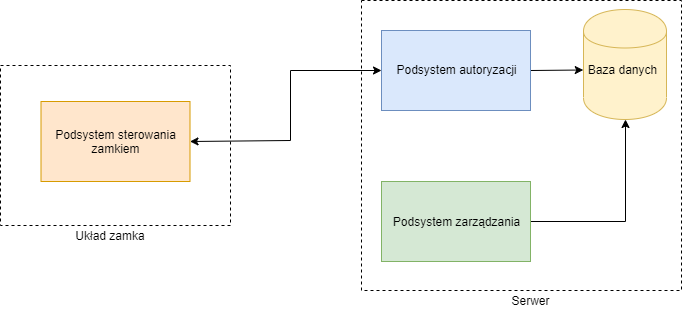
\includegraphics[width=\linewidth]{chapters/images/hl-arch3.png}
                \caption{Architektura systemu}
                \label{fig:hl-arch}
            \end{figure}

            \vspace{10mm} 

            \begin{figure}[h!]
                \centering
                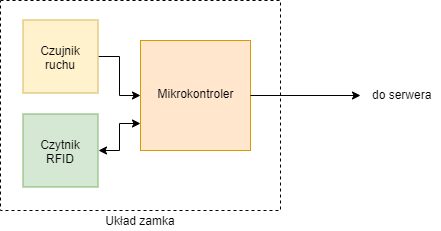
\includegraphics[width=0.5\textwidth]{chapters/images/lock.png}
                \caption{Budowa układu zamka}
                \label{fig:lock-arch}
            \end{figure}

            \begin{figure}[h!]
                \centering
                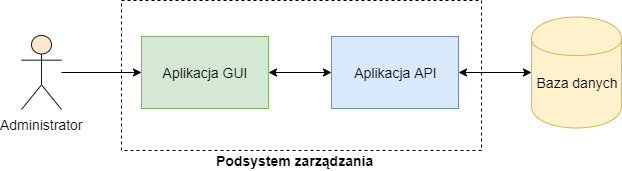
\includegraphics[width=\textwidth]{chapters/images/mngmt_subsystem.png}
                \caption{Budowa podsystemu zarządzającego}
                \label{fig:mngmt_subsystem}
            \end{figure}

        \pagebreak

        \section{Sposób działania}
            Działanie systemu opiera się na współpracy układu zamka z serwerem w celu zapewnienia poprawnej autoryzacji identyfikatorów w zamkach. Funkcjonalność autoryzacji realizowana jest wyłącznie po stronie serwera. Układ zamka, będący urządzeniem klienckim, jest jedynie pośrednikiem przekazującym dane od użytkownika do serwera.

            W celu osiągnięcia największej możliwej wydajności energetycznej czytnik RFID oraz mikrokontroler przez większą część czasu pozostają w stanie uśpienia. Zadaniem czujnika ruchu, zasilanego przez cały czas, jest odpowiednio wczesne wykrycie zbliżającego się użytkownika i wybudzenie mikrokontrolera, który z kolei jest odpowiedzialny za zasilenie czytnika RFID oraz nawiązanie połączenia z serwerem. Jeśli operacja nawiązania połączenia przebiegnie pomyślnie, a do czytnika przyłożony zostanie identyfikator, rozpoczyna się proces przekazywania danych odczytanych z identyfikatora do serwera w celu autoryzacji identyfikatora. Należy zwrócić uwagę na niekorzystne z punktu widzenia systemu warunki, które mogą zajść w trakcie procesu:

            \begin{enumerate}
                \item
                    Jeżeli identyfikator nie zostanie przyłożony w przeciągu 10~sek. od momentu wybudzenia czytnika, mikrokontroler ponownie wprowadza czytnik oraz samego siebie w stan uśpienia.
                \item
                    Jeżeli połączenie z serwerem nie może zostać nawiązane w czasie \textit{t + 3~sek.}, gdzie \textit{t} jest zmiennym czasem upływającym od momentu podjęcia próby nawiązania połączenia z serwerem do momentu zakończenia odczytu danych z identyfikatora, mikrokontroler sygnalizuje użytkownikowi błąd połączenia, po czym wprowadza się w stan uśpienia.
            \end{enumerate}

            Jeżeli żadna z wymienionych wyżej niekorzystnych sytuacji nie wystąpi i dane zostaną pomyślnie przesłane do serwera, serwer podejmuje decyzję o przyznaniu bądź odmowie dostępu. Dokonuje tego po wysłaniu zapytania do bazy danych, a następnie wysyła potwierdzenie lub odmowę do mikrokontrolera. Mikrokontroler w sposób wizualny sygnalizuje decyzję użytkownikowi, a jeżeli była ona pomyślna, dodatkowo wysyła sygnał otwierający zamek. Niezależnie od decyzji serwera, wpis o próbie dostępu zostaje zapisany w bazie danych, skąd może być pobrany przez podsystem zarządzający w celu prezentacji danych administratorowi systemu.

            Opisane wyżej mechanizmy zostały szerzej ukazane na diagramach sekwencji. Diagramy \ref{fig:sequence1}-\ref{fig:sequence3} dotyczą podsystemu sterowania zamkiem oraz podsystemu autoryzacji, natomiast diagramy \ref{fig:sequence4}-\ref{fig:sequence5} dotyczą podsystemu zarządzającego.

            Przedstawione sytuacje to kolejno: proces autoryzacji identyfikatora użytkownika w przypadku najbardziej pomyślnego scenariusza (\ref{fig:sequence1}), przepływ sterowania pomiędzy elementami systemu w sytuacji, gdy użytkownik zostanie wykryty, ale identyfikator nie zostanie przyłożony do czytnika w zadanym przedziale czasu (\ref{fig:sequence2}), przepływ sterowania pomiędzy elementami systemu w sytuacji, gdy niemożliwe jest nawiązanie połączenia z serwerem (\ref{fig:sequence3}), przepływ sterowania pomiędzy warstwami podsystemu zarządzającego w sytuacji żądania dostępu do historii prób dostępu przez administratora systemu (\ref{fig:sequence4}) oraz przepływ sterowania pomiędzy warstwami podsystemu zarządzajacego w sytuacji dodania nowego identyfikatora przez administratora systemu (\ref{fig:sequence5}).

            Należy zwrócić uwagę na możliwość wystąpienia również innych sytuacji niekorzystnych, takich jak błąd połączenia z bazą danych lub \textbf{co jeszcze?}. Ich obsługa jest pomijalna z punktu widzenia współpracy komponentów systemu, dlatego nie została uwzględniona na diagramach.

            \begin{figure}[]
                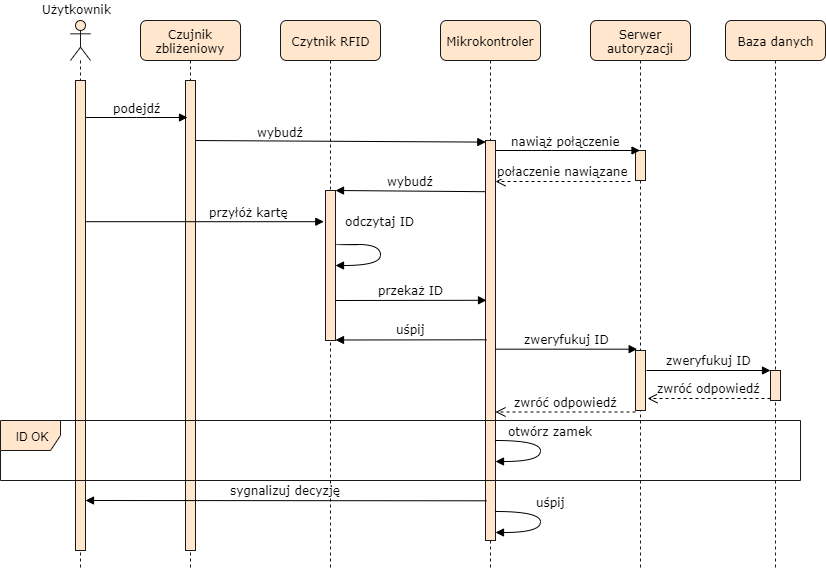
\includegraphics[width=\linewidth]{chapters/images/sequence1.png}
                \caption{Przepływ sterowania w procesie autoryzacji identyfikatora}
                \label{fig:sequence1}
            \end{figure}

            \begin{figure}[]
                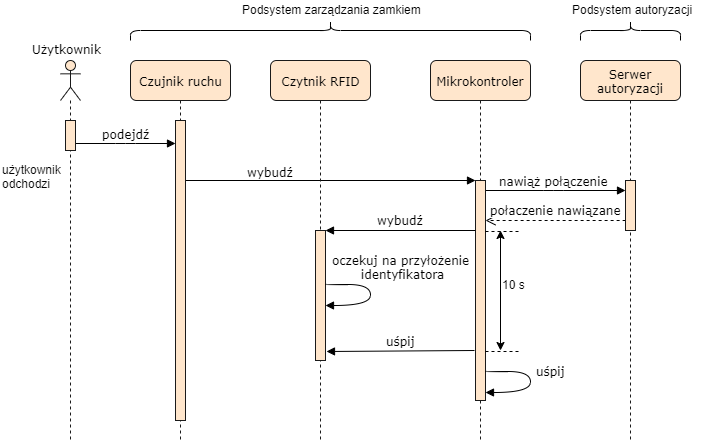
\includegraphics[width=\linewidth]{chapters/images/sequence2.png}
                \caption{Przepływ sterowania w sytuacji wykrycia użytkownika nie prezentującego identyfikatora}
                \label{fig:sequence2}
            \end{figure}

            \begin{figure}[]
                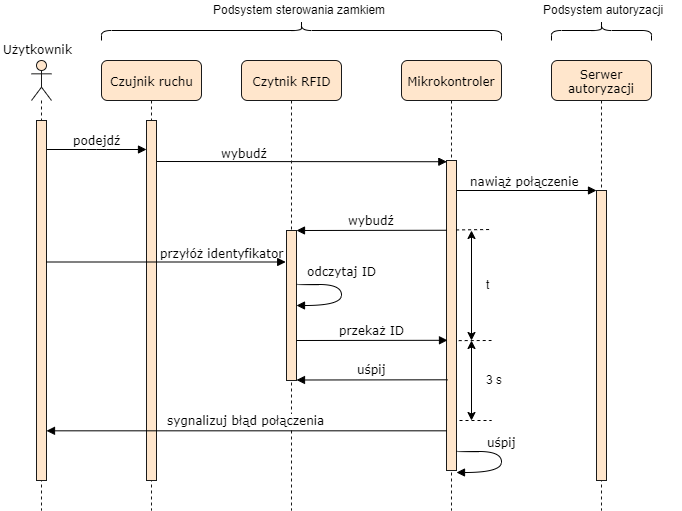
\includegraphics[width=\linewidth]{chapters/images/sequence3.png}
                \caption{Przepływ sterowania w sytuacji braku możliwości nawiązania połączenia z serwerem}
                \label{fig:sequence3}
            \end{figure}

            \begin{figure}[]
                \centering
                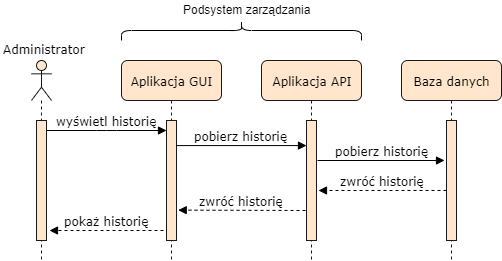
\includegraphics[width=.7\linewidth]{chapters/images/sequence4.png}
                \caption{Przepływ sterowania w procesie żądania dostępu do historii prób dostępu}
                \label{fig:sequence4}
            \end{figure}

            \begin{figure}[]
                \centering
                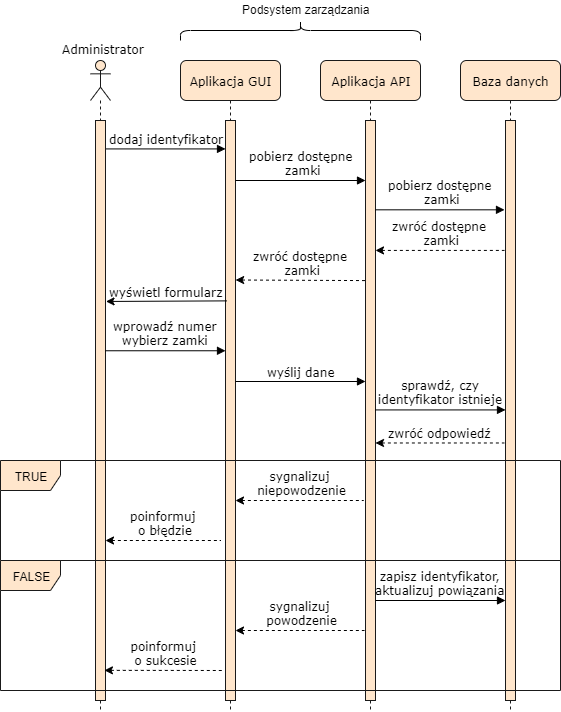
\includegraphics[width=.7\linewidth]{chapters/images/sequence5.png}
                \caption{Przepływ sterowania w procesie dodawania do systemu nowego identyfikatora}
                \label{fig:sequence5}
            \end{figure}


                    

